\documentclass[conference]{IEEEtran}
\IEEEoverridecommandlockouts
% The preceding line is only needed to identify funding in the first footnote. If that is unneeded, please comment it out.
\usepackage{cite}
\usepackage{amsmath,amssymb,amsfonts}
\usepackage{algorithmic}
\usepackage{graphicx}
\usepackage{textcomp}
\usepackage{xcolor}
\def\BibTeX{{\rm B\kern-.05em{\sc i\kern-.025em b}\kern-.08em
    T\kern-.1667em\lower.7ex\hbox{E}\kern-.125emX}}
\begin{document}

\title{CSE453-Pattern Recognition\\
FINAL PROJECT REPORT
}

\author{\IEEEauthorblockN{Berke Süslü}
\IEEEauthorblockA{\textit{Computer Engineering} \\
\textit{161044076}\\
berke.suslu2016@gtu.edu.tr}
}
\maketitle

\section{Introduction}
This project is about using flag attributes in order to guess countries religion.To achieve this, feature selection and classification methods are used.

\section{Dataset}

\subsection{General Information}

The dataset contains details of various nations and their flags. In the dataset, the fields are separated by commas. The dataset is created in 5/15/1990 and has 30 attributes and 194 instances.\cite{b1}

\subsection{Attributes Information}

\begin{table}[htbp]
\begin{center}
\begin{tabular}{ |c|c| } 
 \hline
 Atrribute name & Information about attributes \\
 \hline
 name & Name of the country concerned \\ 
 \hline
 landmass &	1=N.America, 2=S.America, 3=Europe\\
 & 4=Africa, 5=Asia, 6=Oceania \\
 \hline
 zone & Geographic quadrant, based on Greenwich and \\& the Equator:
                		1=NE, 2=SE, 3=SW, 4=NW \\ 
 \hline
 area & in thousands of square km\\
 \hline
 population & in round millions\\
 \hline
 language & 1=English, 2=Spanish, 3=French, 4=German,\\& 5=Slavic, 6=Other 
               		Indo-European, 7=Chinese,\\& 8=Arabic, 
               		9=Japanese/Turkish/Finnish/Magyar,\\& 10=Others\\
 \hline
 religion & 0=Catholic, 1=Other Christian, 2=Muslim,\\& 3=Buddhist, 4=Hindu,
               		5=Ethnic, 6=Marxist,\\& 7=Others\\
 \hline
 bars & Number of vertical bars in the flag\\
 \hline
 stripes & Number of horizontal stripes in the flag\\
 \hline
 colours & Number of different colours in the flag\\
 \hline
 red & 0 if red absent, 1 if red present in the flag\\
 \hline
 green & same for green\\
 \hline
 blue & same for blue\\
 \hline
 gold & same for gold(also yellow)\\
 \hline
 white & same for white\\
 \hline
 black & same for black\\
 \hline
 orange & same for orange\\
 \hline
 mainhue & predominant colour in the flag\\ 
 \hline
 circles & Number of circles in the flag\\
 \hline
 crosses & Number of (upright) crosses\\
 \hline
 saltires & Number of diagonal crosses\\
 \hline
 quarters & Number of quartered sections\\
 \hline
 sunstars & Number of sun or star symbols\\
 \hline
 crescent & 1 if a crescent moon symbol present, else 0\\
 \hline
 \end{tabular}
\end{center}
\end{table}
\begin{table}[htbp]
\begin{center}
\begin{tabular}{ |c|c| } 
 \hline
 triangle & 1 if any triangles present, 0 otherwise\\
 \hline
 icon & 1 if an inanimate image present \\& (e.g., a boat), otherwise 0\\
 \hline
 animate & 1 if an animate image \\& (e.g., an eagle, a tree, a human hand)\\& present, 0 otherwise\\
 \hline
 text & 1 if any letters or writing on \\& the flag (e.g., a motto or\\& slogan), 0 otherwise\\
 \hline
 topleft & colour in the top-left corner\\
 \hline
 botright & Colour in the bottom-left corner\\
 \hline
\end{tabular}
\end{center}
\end{table}

\section{Feature Selection Methods}
The following methods were used for feature selection.
\renewcommand{\theenumi}{\alph{enumi}}
\begin{enumerate}
    \item ANOVA Test
    \item Chi-squared Test
    \item Recursive Feature Elimination
\end{enumerate}
The following table was used when deciding on these methods.
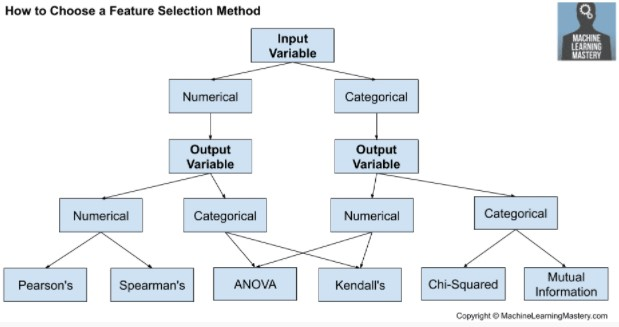
\includegraphics[scale=0.5]{featureselection.jpg}\cite{b2}

\subsection{ANOVA Test}
Analysis of variance (ANOVA) is a collection of statistical models and their associated estimation procedures (such as the "variation" among and between groups) used to analyze the differences among means. ANOVA was developed by the statistician Ronald Fisher. ANOVA is based on the law of total variance, where the observed variance in a particular variable is partitioned into components attributable to different sources of variation. In its simplest form, ANOVA provides a statistical test of whether two or more population means are equal, and therefore generalizes the t-test beyond two means.\cite{b3} ANOVA test was used to obtain categorical outputs from numerical inputs. The test produced p-values and a significance level of 0.05 was set. The features below the significance level were selected.
Selected features:"population", "colours", "circles", "crosses", "saltires", "quarters".

\subsection{Chi-squared Test}
A chi-squared test, also written as $X^2$ test, is a statistical hypothesis test that is valid to perform when the test statistic is chi-squared distributed under the null hypothesis, specifically Pearson's chi-squared test and variants thereof. Pearson's chi-squared test is used to determine whether there is a statistically significant difference between the expected frequencies and the observed frequencies in one or more categories of a contingency table.\cite{b4} Chi-squared test was used to obtain categorical outputs from categorical inputs. The test produced p-values and a significance level of 0.05 was set. The features below the significance level were selected.
Selected features:"landmass", "zone", "language", "green", "blue", "crescent".

\subsection{Recursive Feature Elimination}
Given an external estimator that assigns weights to features (e.g., the coefficients of a linear model), the goal of recursive feature elimination (RFE) is to select features by recursively considering smaller and smaller sets of features. First, the estimator is trained on the initial set of features and the importance of each feature is obtained either through any specific attribute or callable. Then, the least important features are pruned from current set of features. That procedure is recursively repeated on the pruned set until the desired number of features to select is eventually reached.\cite{b5}
The Recursive Filter Elimination method was used to combine the results from the two feature selection methods. Decision Tree Classifier was used as the estimator. The best 10 features are selected.\\
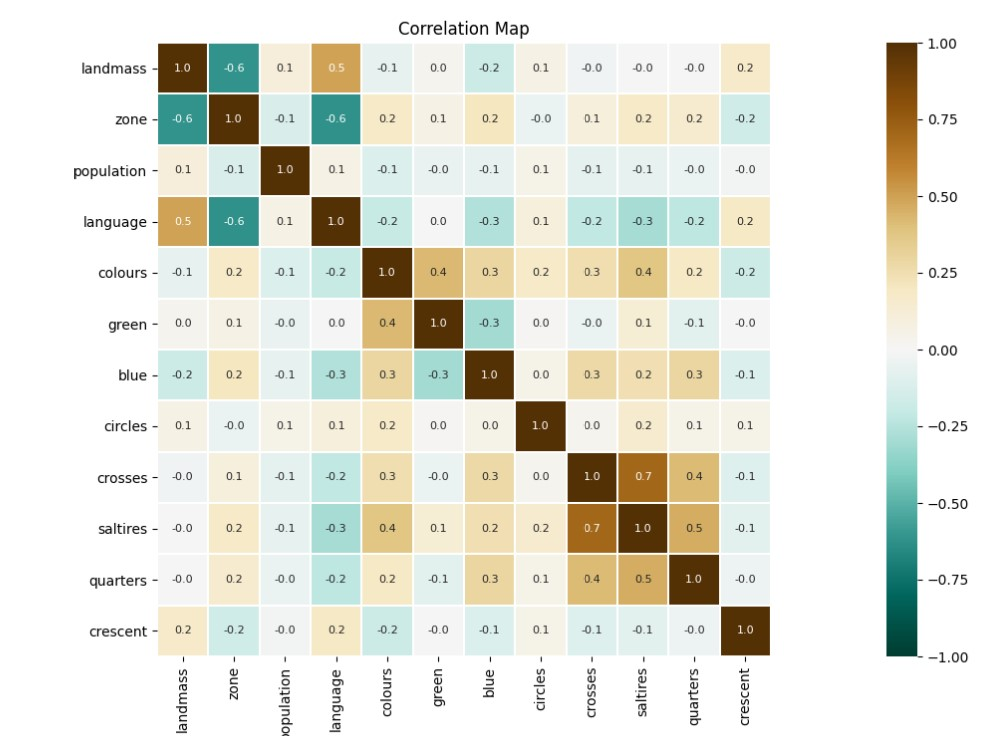
\includegraphics[scale=0.35]{corr.jpg}

\section{Classification}
\subsection{Decision Tree Classifier}
Decision Trees (DTs) are a non-parametric supervised learning method used for classification and regression. The goal is to create a model that predicts the value of a target variable by learning simple decision rules inferred from the data features. A tree can be seen as a piecewise constant approximation.\cite{b6}
Decision trees learn from data to approximate a sine curve with a set of if-then-else decision rules. The deeper the tree, the more complex the decision rules and the fitter the model. Entropy is used as a classification criteria. The obtained features were loaded into the Decision Tree model and the training data were placed in this model($\%80$ training data, $\%20$ test data). After the model was created, predictions were made with the test values and compared with the actual values. Example of a decision tree model:

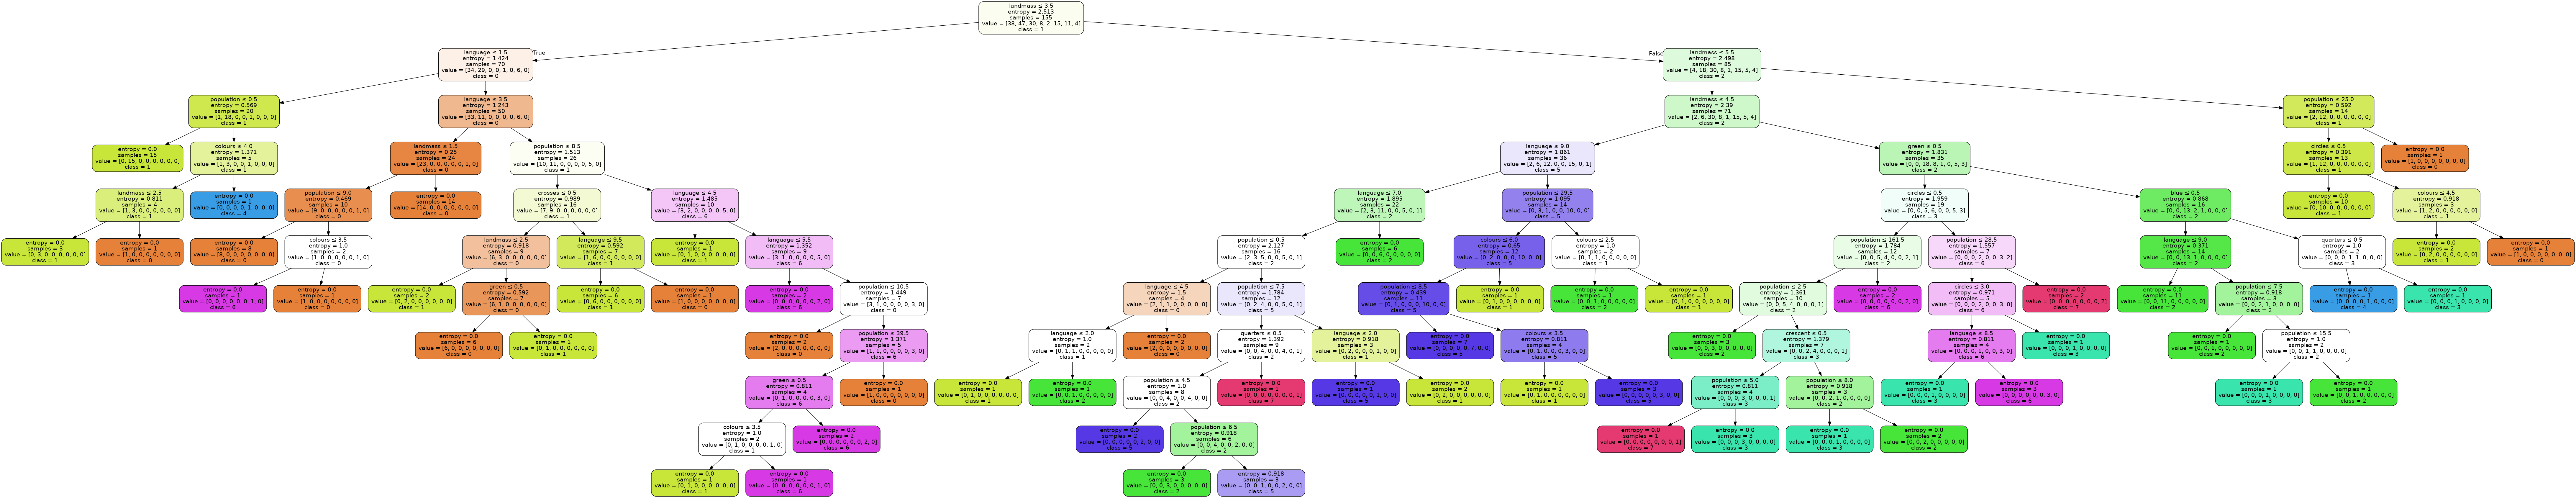
\includegraphics[scale=0.03]{rfe_decision_tree.png}


\section{Conclusion}

The test and training data were shuffled so that the results were different each time. As a result, the accuracy rate varies between $\%50$ and $\%80$. This means that the probability of finding the right religion from the predictions is higher than $\%50$.

\begin{thebibliography}{9}



\bibitem{b1} 
UCI Machine Learning Repository: Flags Data Set\\
George H. John and Ron Kohavi and Karl Pfleger.\\
Irrelevant Features and the Subset Selection Problem. ICML. 1994.
\\\texttt{https://archive.ics.uci.edu/ml/datasets/Flags}


\bibitem{b2} 
How to Choose a Feature Selection Method For Machine Learning
\\\texttt{https://machinelearningmastery.com/feature-selection-\\with-real-and-categorical-data/}

\bibitem{b3} 
Wikipedia - Analysis of Variance
\\\texttt{https://en.wikipedia.org/wiki/Analysis\_of\_variance}

\bibitem{b4} 
Wikipedia - Chi-squared test
\\\texttt{https://en.wikipedia.org/wiki/Chi-squared\_test}

\bibitem{b5} 
SKLearn Manual - RFE
\\\texttt{https://scikit-learn.org/stable/modules/generated/\\sklearn.feature\_selection.RFE.html}

\bibitem{b6} 
SKLearn - Decision Trees
\\\texttt{https://scikit-learn.org/stable/modules/tree.html}



\end{thebibliography}

\vspace{12pt}
\end{document}
